Nesta seção, apresentamos os resultados do nosso experimento de amostragem de sinais. A Figura~\ref{fig:input-signal}. mostra o sinal de entrada original, que serve como base para a aplicação das diferentes métodos de amostragem: ideal, natural e flat-top.

A análise deste sinal de entrada é crucial para entender a qualidade do sinal original e sua estrutura antes da modulação e amostragem. Observando a Figura~\ref{fig:input-signal}, podemos identificar as características principais do sinal que serão importantes para avaliar o impacto das técnicas de amostragem em etapas subsequentes.

Este sinal inicial será comparado com os sinais amostrados resultantes das técnicas aplicadas, permitindo uma análise detalhada das mudanças introduzidas durante o processo de amostragem e modulação.

\begin{figure}[H]
    \centering
    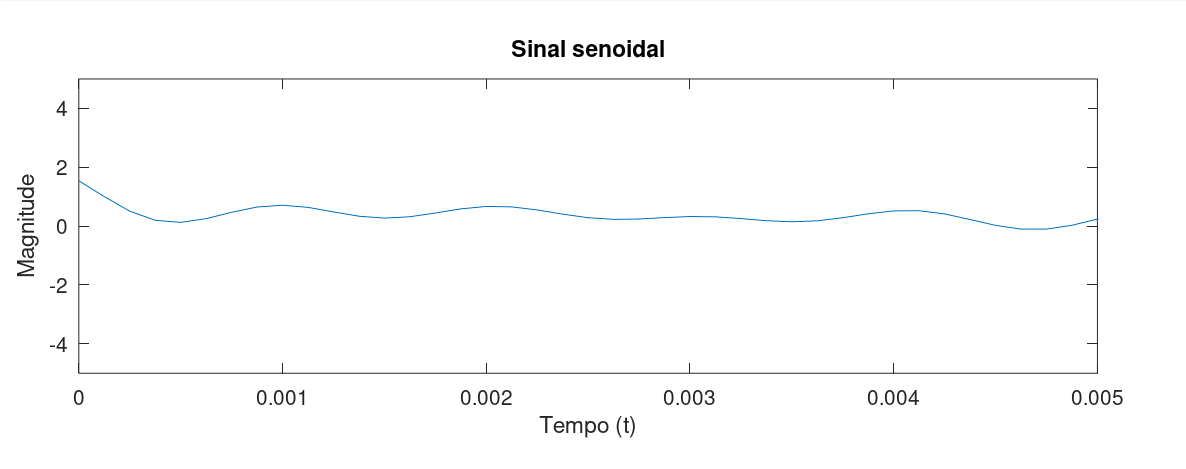
\includegraphics[width=1\linewidth]{03_results/octave_results/sinal_senoidal.png}
    \caption{Sinal senoidal de entrada}
    \label{fig:input-signal}
\end{figure}

\subsection{Ideal}

Na primeira parte da Figura~\ref{fig:ideal-pam}, observamos o sinal de trem de impulsos gerados, apresentados de forma discreto. O trem de impulsos é gerado para modular o sinal de entrada original e possibilitar a aplicação da amostragem com método ideal. Este trem é caracterizado teoricamente como conjunto infinito de impulsos unitários, de delta de dirac ($\delta$), espaçados de uma unidade, conforme a equação  \ref{tremimpulsos}. 

Após a geração do trem de impulsos, realizamos sua multiplicação junto ao sinal original, levando ao sinal como ilustrado na figura~\ref{fig:ideal-pam}, com \textit{aliasing} e na figura \ref{fig:ideal-pam-aliasing}, sem \textit{aliasing}. Esse processo resulta em um sinal modulado que reflete a amostragem do sinal original em intervalos discretos. 

Para realizar a execução das amostragens, foi necessário realizar a definição de uma frequência de amostragem, a qual é necessária para cada um dos métodos de amostragem apresentados conseguirem obter os valores corretos. Para a definição da frequência de amostragem, foi levada em consideração os valores retornados pelo código, dentre eles, o principal utilizado foi o valor da frequência máxima utilizada. Sendo $f_{max} = 910Hz; $
$F_s Nyquist = 2002Hz;$
$Aliasing F_s = 819Hz.$

\begin{figure}[H]
    \centering
    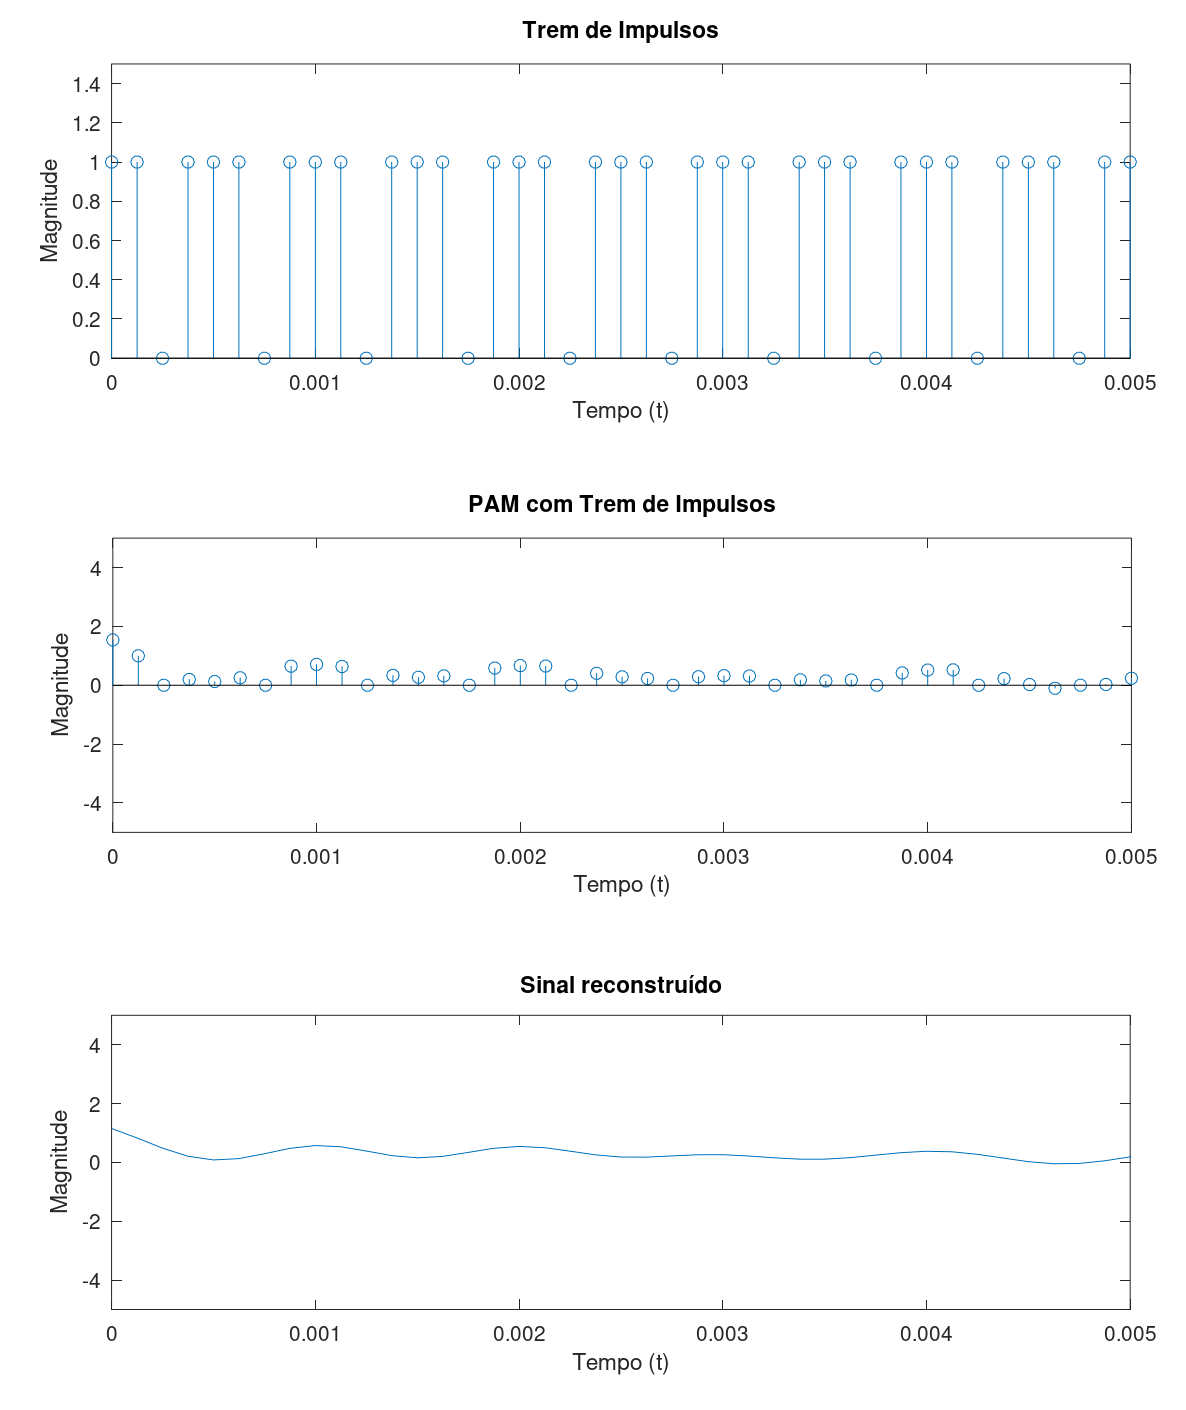
\includegraphics[width=0.8\linewidth]{03_results/octave_results/ideal_sampling.png}
    \caption{Saída sem Aliasing da amostragem Ideal}
    \label{fig:ideal-pam}
\end{figure}

\begin{figure}[H]
    \centering
    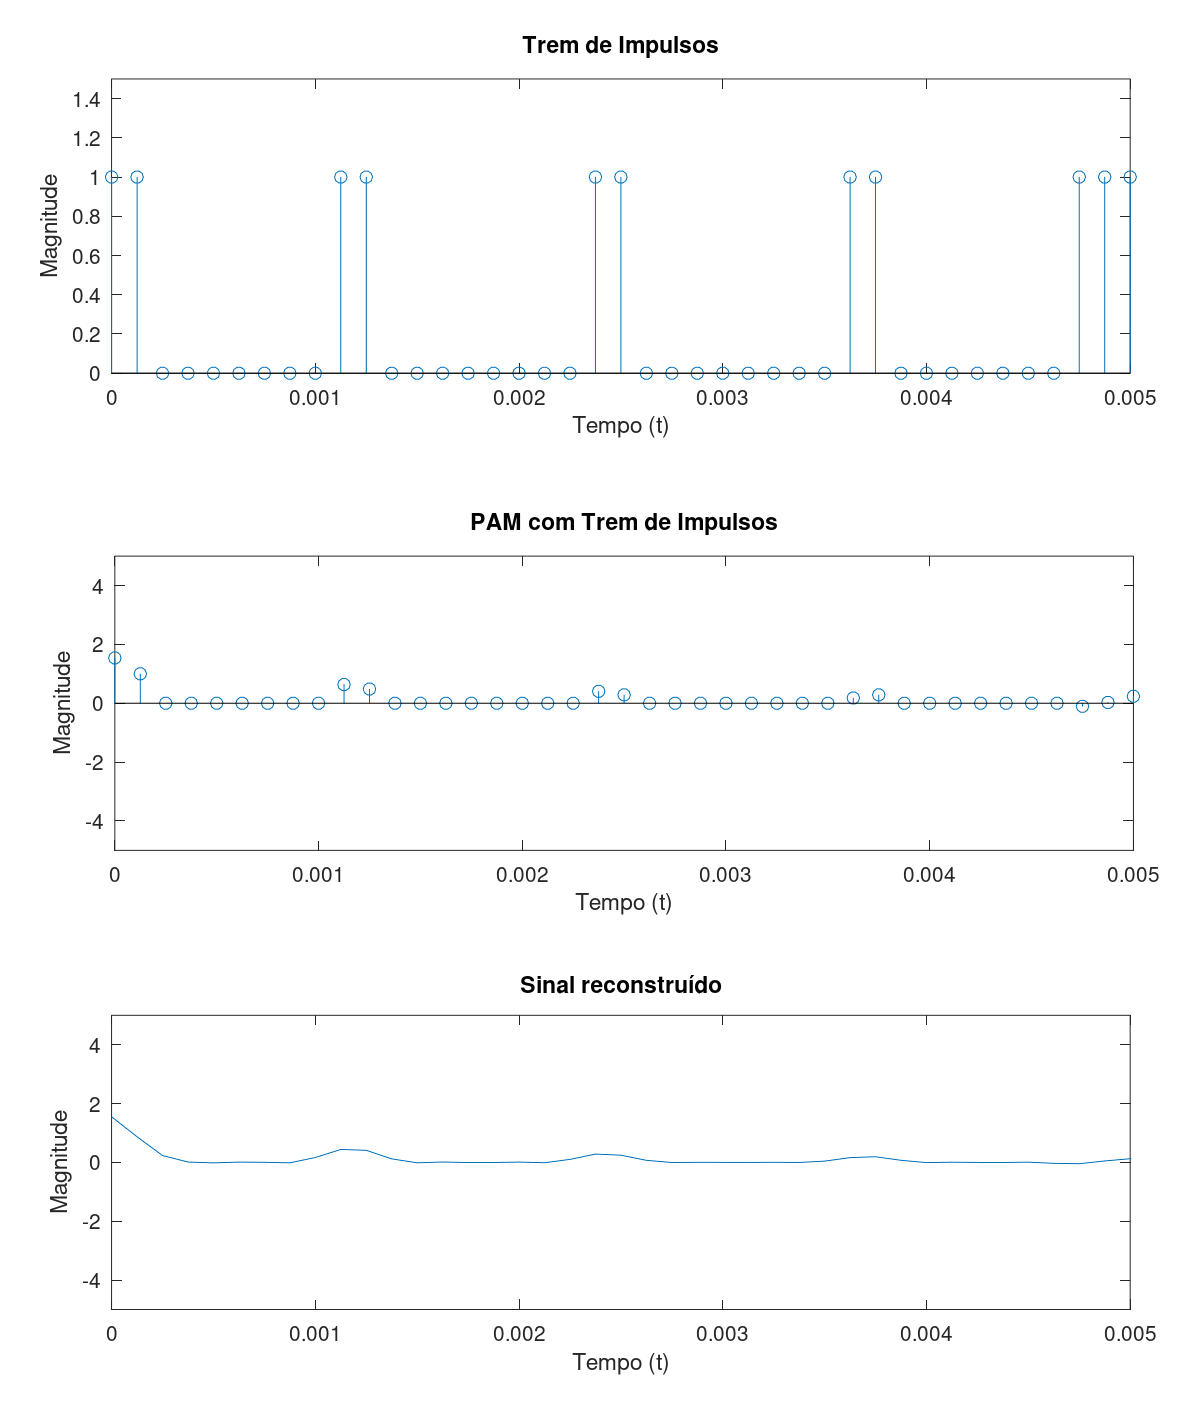
\includegraphics[width=0.8\linewidth]{03_results/octave_results/ideal_aliasing_sampling.png}
    \caption{Saída da amostragem Ideal - Frequencia de Amostragem = 819}
    \label{fig:ideal-pam-aliasing}
\end{figure}

\subsection{Natural}

Na Figura~\ref{fig:natural-pam}, observamos na primeira parte o trem de pulsos retangulares. Após gerado esse trem de pulsos, esse sinal foi multiplicado ao sinal original, gerando o sinal amostrado pelo método natural, como é possível observar na Figura~\ref{fig:natural-pam}. A amostragem onde acontece aliasing é possível observar na Figura~\ref{fig:natural-pam-aliasing}.

\begin{figure}[H]
    \centering
    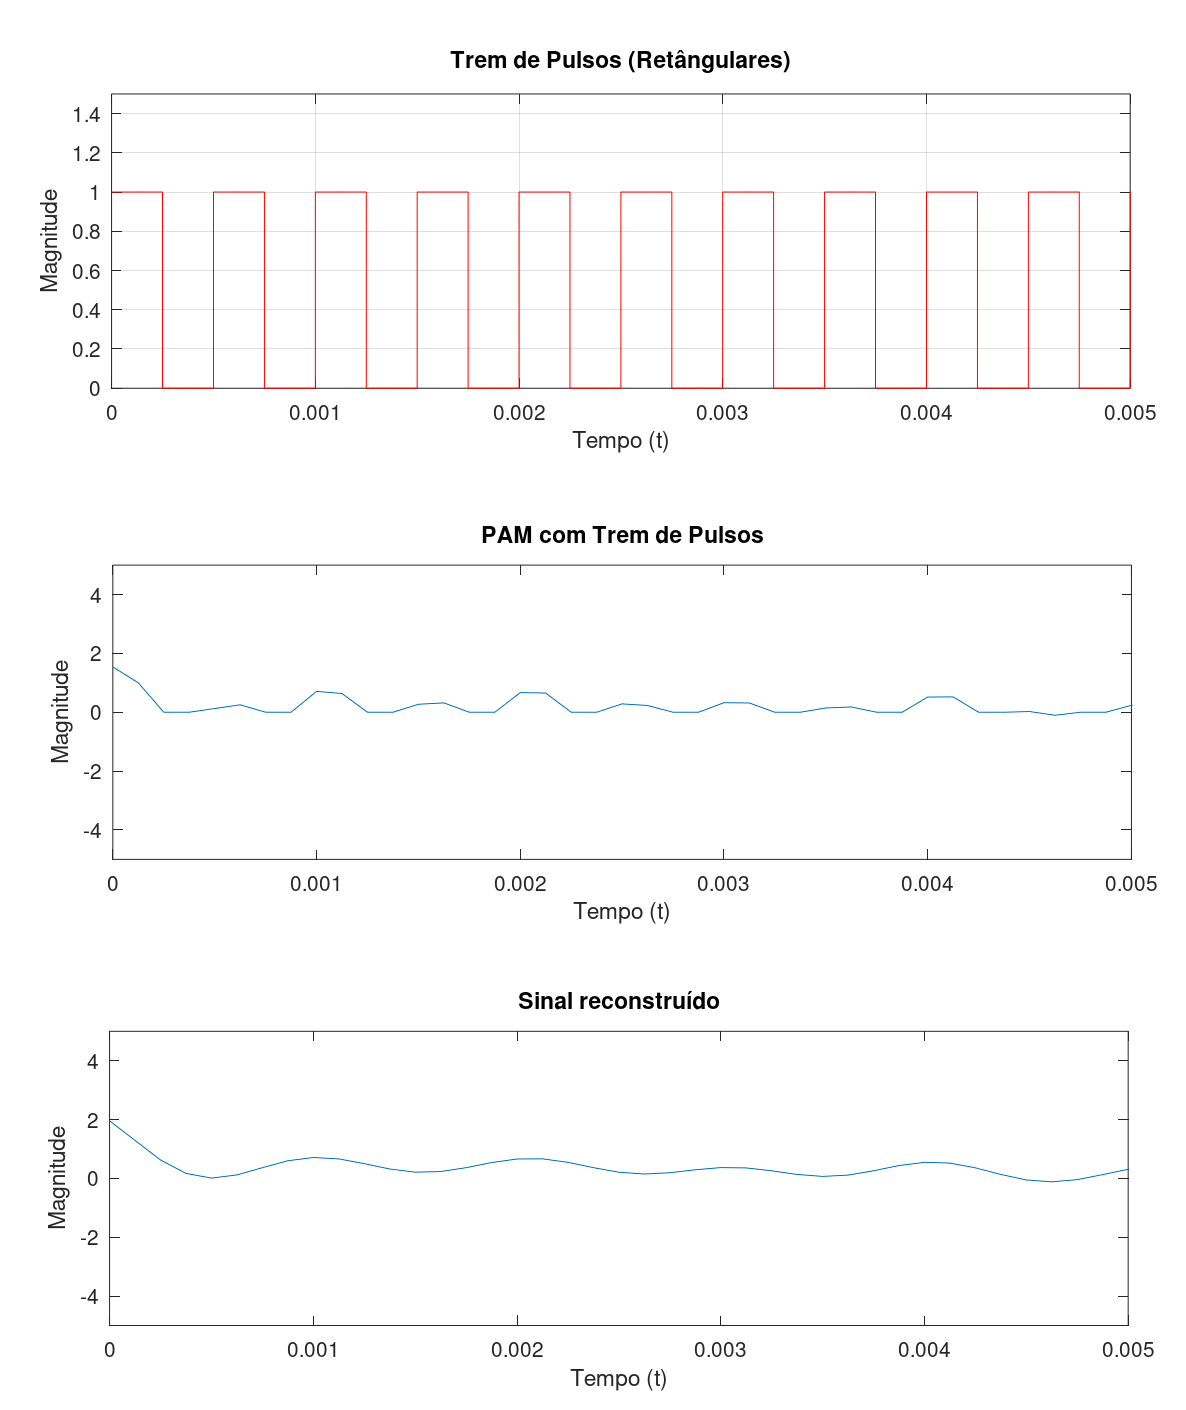
\includegraphics[width=0.8\linewidth]{03_results/octave_results/natural_sampling.png}
    \caption{Saída sem Aliasing da amostragem Natural}
    \label{fig:natural-pam}
\end{figure}

\begin{figure}[H]
    \centering
    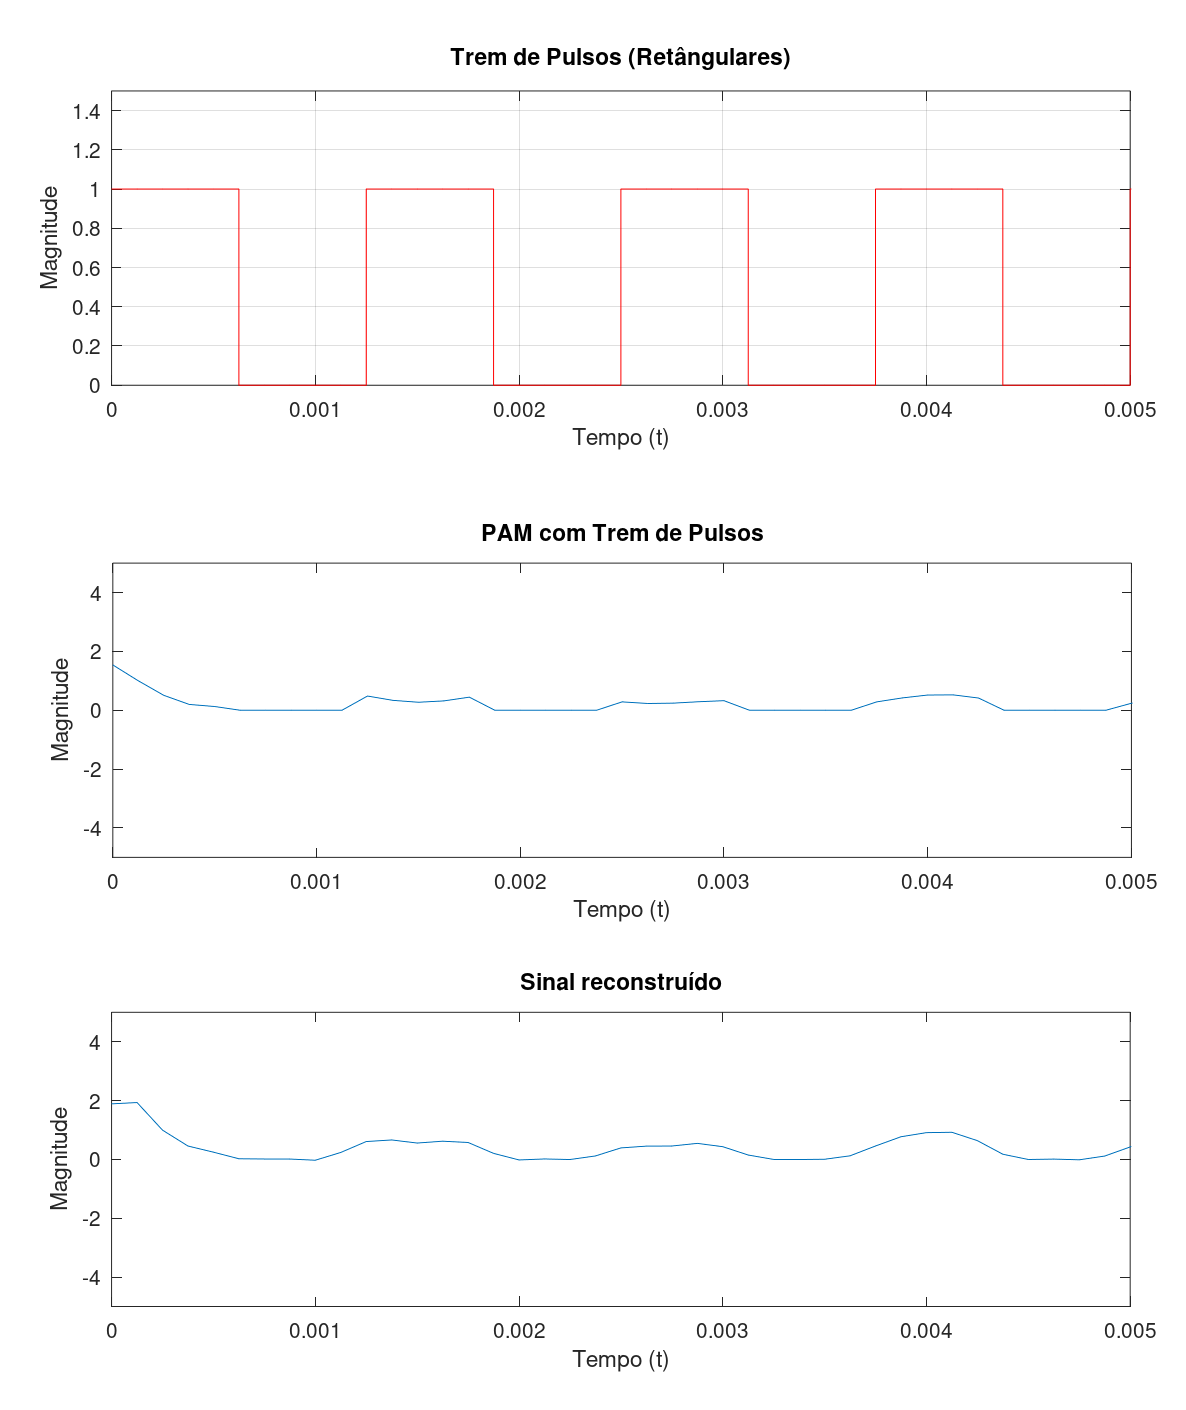
\includegraphics[width=0.8\linewidth]{03_results/octave_results/natural_aliasing_sampling.png}
    \caption{Saída da amostragem Natural - Frequencia de Amostragem = 819}
    \label{fig:natural-pam-aliasing}
\end{figure}

\subsection{Flat-Top}

Assim como na amostragem natural, é utilizado o trem de pulsos para realizar a modulação do sinal, como observado na Figura~\ref{fig:flattop-pam}. Mas, diferente da abordagem natural, no método de topo plano o trem de pulsos, quando modulado,  manterá o valor da amostragem até o próximo intervalo de amostragem $\tau$, conforme descrito no desenvolvimento das equações de \ref{eq:flattopFT} a  \ref{eq:flattop}. Os valores obtidos quando se tem \textit{aliasing} é possível observar na Figura~\ref{fig:flattop-pam-aliasing}.
\begin{figure}[H]
    \centering
    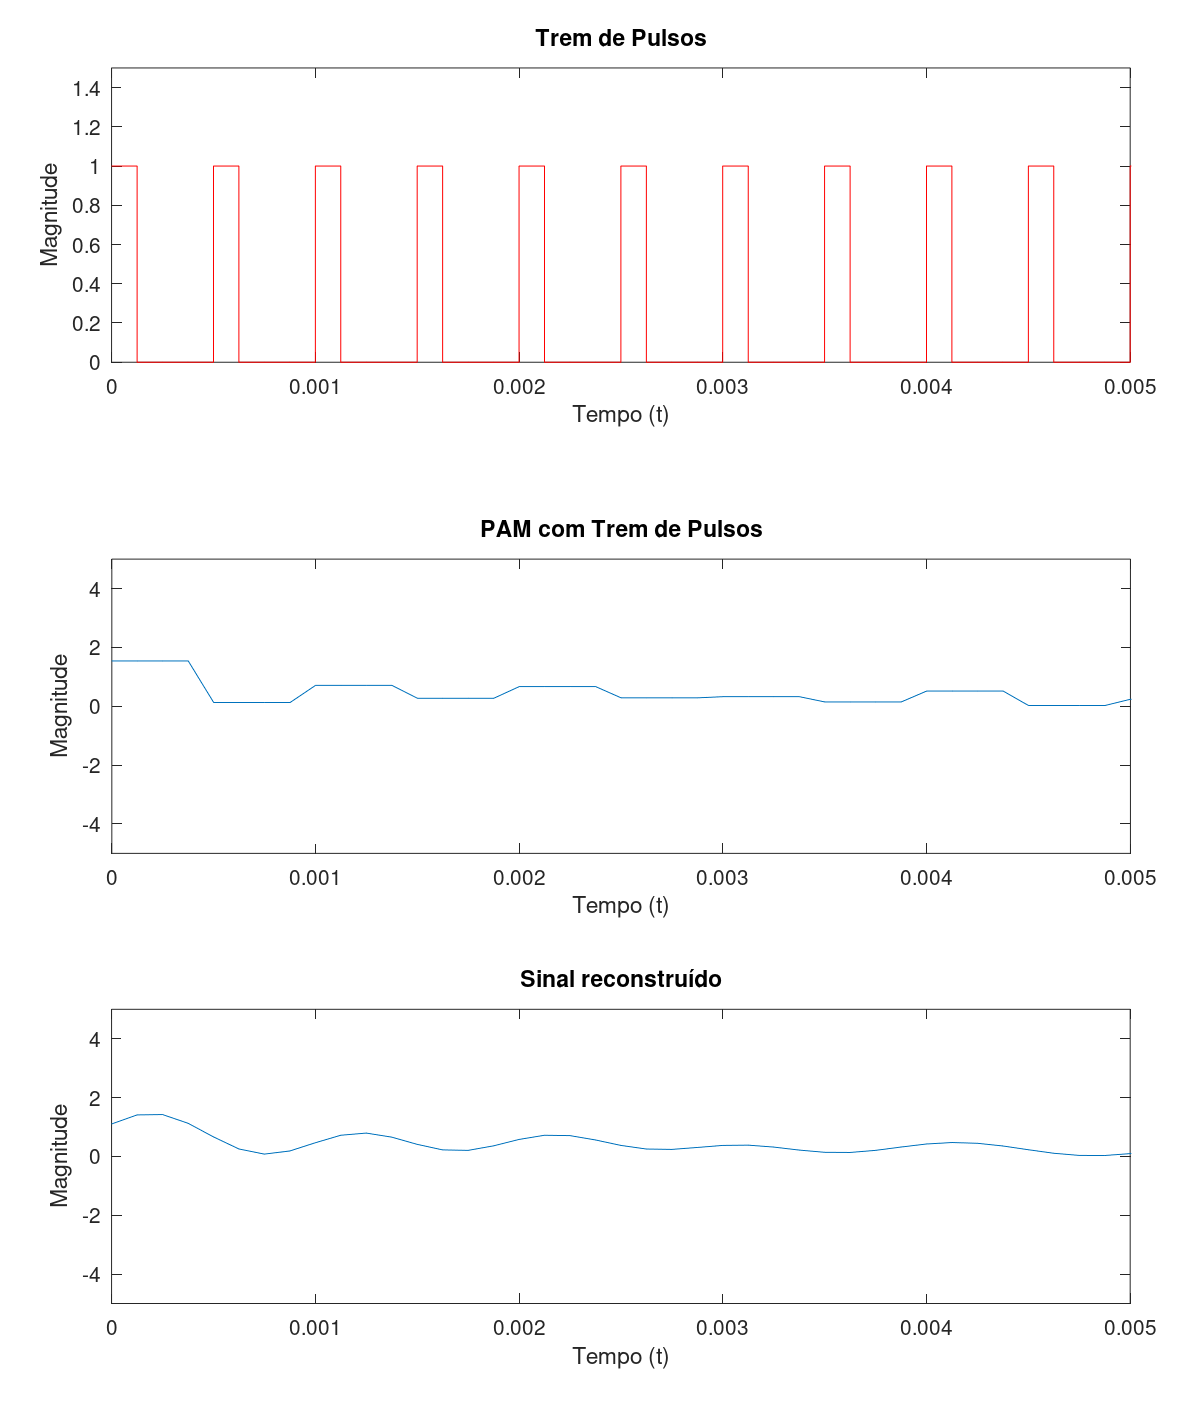
\includegraphics[width=0.8\linewidth]{03_results/octave_results/flattop_sampling.png}
    \caption{Saída sem Aliasing da amostragem Flat-Top}
    \label{fig:flattop-pam}
\end{figure}

\begin{figure}[H]
    \centering
    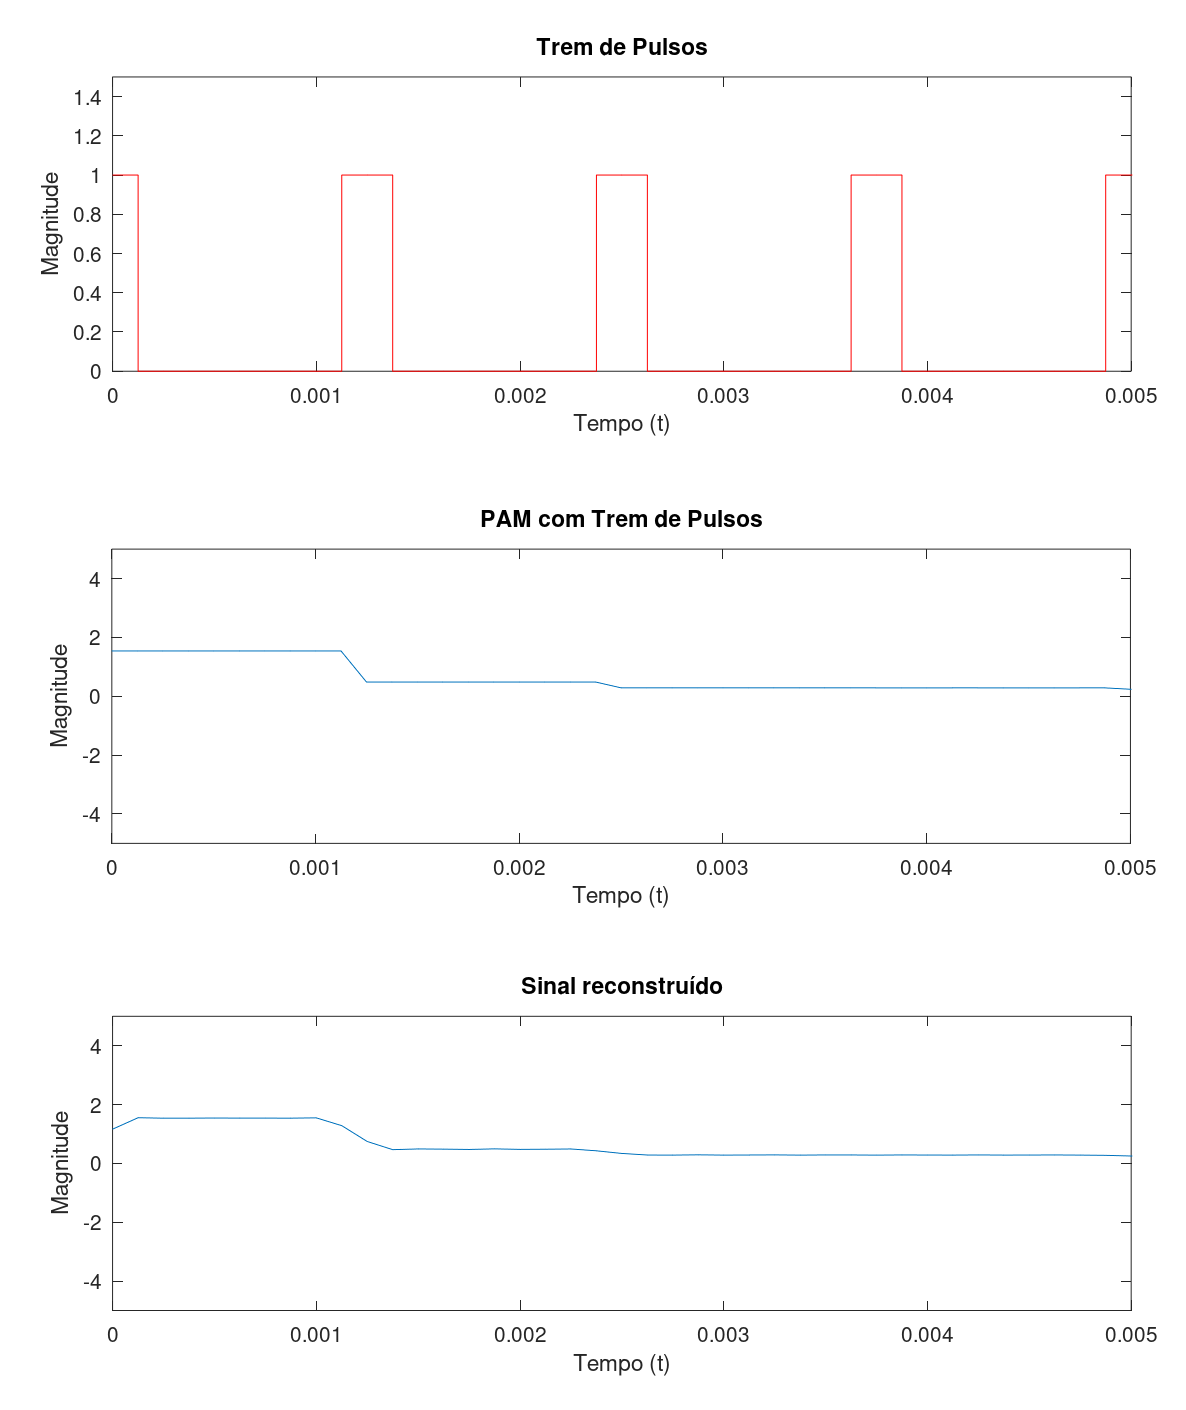
\includegraphics[width=0.8\linewidth]{03_results/octave_results/flattop_aliasing_sampling.png}
    \caption{Saída da amostragem Flat-Top - Frequência de Amostragem = 819}
    \label{fig:flattop-pam-aliasing}
\end{figure}

Nos três métodos de amostragem, quando a frequência de amostragem possui o valor abaixo do ideal, acontece o aliasing, resultando em um sinal reconstruído que não corresponde com o sinal original, resultando em perda de informações do sinal. Essa situação podendo ser vista na Figura~\ref{fig:ideal-pam-aliasing}, Figura~\ref{fig:natural-pam-aliasing} e Figura~\ref{fig:flattop-pam-aliasing}


